\documentclass[addpoints]{exam}
\usepackage{url}
\usepackage{amsmath,amsthm,enumitem}
\usepackage{amssymb}
\usepackage{graphicx}
\usepackage{qtree}
\usepackage[nodayofweek,level]{datetime}
\usepackage{color}
\usepackage{csquotes}
\usepackage{pgf, tikz}
\usetikzlibrary{arrows, automata}
\usepackage{algorithm,algpseudocode}
\usepackage{graphicx}
\usetikzlibrary{positioning}
\usetikzlibrary{calc,arrows.meta,positioning}

\tikzset{
    every node/.style={font=\sffamily\small},
    main node/.style={thick,circle,draw,font=\sffamily\Large}
}
\newtheorem*{claim}{Claim}
\definecolor{qcolor}{rgb}{0, 0, 0.3}
\definecolor{acolor}{rgb}{0, 0, 0}
%\input myfonts
\qformat{Question \thequestion: \thequestiontitle\dotfill \textbf{[\totalpoints]}}
\pointname{}
\bonuspointname{}
\pointformat{[\bfseries\thepoints]}

\lhead{Gopal Menon (u0772360)}
\chead{\bf{HW3}}
\rhead{CS 6150 \today}
\headrule

\begin{document}

\section*{Collaborators}

Ben Nelson and I collaborated for this assignment.

\begin{questions}

\titledquestion{Negative edges}[4]
We saw that Dijkstra's algorithm (as such) requires all the edge weights to be non-negative in order to work. A student suggests a simple fix. Given a graph $G$ with negative weight edges (but no negative cycles), he suggests computing the least weight $w_{\min}$, and then adding $|w_{\min}|$ to all the edge weights. This would make all the weights non-negative. He claims that finding the shortest path on this new graph yields the shortest path in $G$ as well.

Is there something wrong in the reasoning above? Explain with an example (of some fixed size).

\begin{center}
  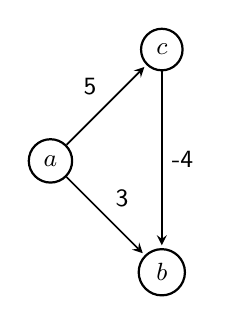
\begin{tikzpicture}[
            > = stealth, % arrow head style
            shorten > = 1pt, % don't touch arrow head to node
            auto,
            node distance = 2cm, % distance between nodes
            semithick % line style
        ]

        \tikzstyle{every state}=[
            draw = black,
            thick,
            fill = white,
            minimum size = 4mm
        ]

        \node[state] (a) {$a$};
        \node[state] (b) [below right of=a] {$b$};
        \node[state] (c) [above right of=a] {$c$};

        \path[->] (a) edge node {3} (b);
        \path[->] (a) edge node {5} (c);
        \path[->] (c) edge node {-4} (b);

  \end{tikzpicture}
\end{center}

Consider the case shown above where we need to find the shortest path from node $a$ to node $b$. The edge lengths are shown next to the edges. It can be seen that the shortest path from $a$ to node $b$ is through $c$, with a length of $5+(-4)=1$. The $1$-hop path from $a$ to $b$ is longer with a length of $3$. If we add $|w_{\min}| = |-4| =4$ to each each, we get the new graph shown below.

\begin{center}
  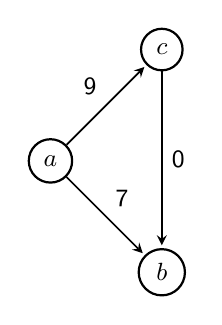
\begin{tikzpicture}[
            > = stealth, % arrow head style
            shorten > = 1pt, % don't touch arrow head to node
            auto,
            node distance = 2cm, % distance between nodes
            semithick % line style
        ]

        \tikzstyle{every state}=[
            draw = black,
            thick,
            fill = white,
            minimum size = 4mm
        ]

        \node[state] (a) {$a$};
        \node[state] (b) [below right of=a] {$b$};
        \node[state] (c) [above right of=a] {$c$};

        \path[->] (a) edge node {7} (b);
        \path[->] (a) edge node {9} (c);
        \path[->] (c) edge node {0} (b);

  \end{tikzpicture}
\end{center}

The shortest path now becomes the one directly from $a$ to $b$. The reason why this fix does not work is that $|w_{\min}|$ is added to each edge length and this may cause the shortest path in the original graph to no longer be the shortest one in the new graph with the changed edge weights, when the shortest path consists of multiple hops and the weight of each hop goes up by $|w_{\min}|$.

\titledquestion{Fattest path}[6]
Let $G$ be a directed graph in which every edge $e$ has a {\em thickness} $t_{e}$.  Given $u$ and $v$, find the path from $u$ to $v$ that maximizes the least-thick-edge on the path. [i.e., we want a path in which {\em every} edge is as thick as possible. Note that the length of the path does not matter.]

You will get partial credit if your algorithm runs in polynomial$(m, n)$ time ($m$ and $n$ are the number of edges and vertices, as usual). To receive full credit, it should run in $O((m+n)\log n)$ time. [{\em Hint: } You might want to modify Dijkstra's algorithm and use its run time analysis as a blackbox.]

\begin{minipage}{\linewidth}
  \begin{algorithm}[H]
    \caption{Modified Dijkstra's Algorithm}\label{Djk}
    \begin{algorithmic}[1]
      \Procedure{ModifiedDijkstra'sAlgorithm}{graph $G \{V, E\}$, thickness\_function $w$, start\_node $s$}
      	\State InitializeGraph($G$,$s$)
	\State $visited\_nodes\_set =\emptyset$
	\State $max\_priority\_q = G.V$ \Comment{based on vertex least thick edge}
	\While {$max\_priority\_q \neq \emptyset$}
		\State $a=Extract\_Max(max\_priority\_q)$
		\State $visited\_nodes\_set =  visited\_nodes\_set \cup \{a\}$
		\For {each vertex $b \in \{ \text{neighbors of  } a$\}}
			\State Relax($a, b, w$)
		\EndFor
	\EndWhile
      \EndProcedure    
      \Procedure{InitializeGraph}{graph $G \{V, E\}$, start\_node $s$}
	\For {each vertext $a \in G.V$}
		\State $a.least\_thick\_edge = 0$
		\State $a.predecessor = NIL$
	\EndFor
	\State $s.least\_thick\_edge =\infty$
      \EndProcedure
      \Procedure{Relax}{current\_node $a$, unvisited\_neighbor $b$, thickness\_function $w$}
	\If {$b.least\_thick\_edge < w(a,b)$}
		\State $b.least\_thick\_edge = w(a,b)$
		\State $b.predecessor = a$
	\EndIf
      \EndProcedure    
     \end{algorithmic}
  \end{algorithm}
\end{minipage}\\\\

The algorithm shown above is a slightly modified version of Dijkstra's Algorithm \cite{CLRS}. All the edges are first initialized with $0$ as the value of the least thick edge on the path that they are on. The starting node is initialized with $\infty$ for the least thick edge. The set of visited nodes is initially empty. A max priority queue based on the least thick edge for each vertex is used. The algorithm then repeatedly extracts the max node from the priority queue which will contain the frontier of unvisited nodes. The extracted node will be the one that lies on the path with the maximum least thickest edge. The running time of this algorithm will be the same \cite{CLRS} as the one for Dijkstra's Algorithm $O(n+m)\log n$.


\titledquestion{Answering distance queries}
Let $G = (V, E)$ be an {\em undirected} graph with all edge weights equal to $1$. Let $d(i,j)$ denote the length of the shortest path between $i$ and $j$.  Now, suppose we wish to answer queries from the user of the kind ``what is $d(u, v)$''? for different $u, v$.

One option is to compute answers to each query as it comes. This takes $O(m+n)$ time using BFS, as the graph is unweighted.  Another option is to solve the so-called All-Pairs-Shortest-Path (APSP) problem and store all the answers. This returns the answer in $O(1)$ time, but uses $O(n^2)$ additional memory -- which can be cumbersome for large graphs (think $n = 10^8$ -- common in real networks).  The goal of this problem is to see if there is middle ground, if we allow {\em an approximation}. The proposed algorithm does the following:

(pre-processing): choose a random subset $S$ of vertices (the size is specified later). For each $s \in S$, do a BFS and store the values $d(s, u)$ for all $u \in V$.

(query): at query time, given $u, v$, return $\min_{s \in S} \{ d(u, s) + d(v, s) \}$. 

\begin{parts}
\part[2] Prove that for any choice of $S$, the value we output for a query is $\ge d(u, v)$.  
\part[3] Suppose we obtain $S$ by randomly including every vertex of $U$ with probability $r/n$. (Thus the expected size of $S$ is $r$.) What are the expected pre-processing time and the memory usage of the algorithm?
\part[7] Suppose that $d(u,v) > 5n/r$ for some pair of vertices $u,v$.  Prove that with probability $> 0.99$, we obtain the right answer to the distance query. [{\em Hint:} consider the shortest path from $u$ to $v$ and the vertices on it.]
\end{parts}

The moral is that if $G$ is sparse, then by picking say $r = \sqrt{n}$, we can do much better than APSP, and get right distance values for all the ``long paths'' with high probability.

\begin{parts}

\part For any $u$ and $v$, the shortest path between them may or may not include a vertex that is in $S$. In the case that the shortest path between them includes a vertex in $S$, then  
$\min_{s \in S} \{ d(u, s) + d(v, s) \}$ will be equal to $d(u, v)$ for the case when the $s \in S$ that is in the shortest path between $u$ and $v$ is considered. For the case where the shortest path between $u$ and $v$ does not include a vertex in $S$, a path between $u$ and $v$ through any $s \in S$ will be longer than the shortest path between them. So we can conclude that the query will always output a value $\ge d(u, v)$.

\part Assuming that it takes constant time to decide whether to pick a vertex for the set $S$ or not, it will take $O(n)$ to look at every vertex and decide whether to include it or not. For every vertex $s \in S$, we would need to do a BFS in $O(m+n)$ time and then compute and store $d(s,u)$ for every $u \in V$. This will take a total of $O( n  + r \times (m+n)) = O(r \times (m+n))$ time and will need $O(n \times |S|)=O(n \times r)$ storage to store the distance to each of the $n$ vertices from every vertex $s \in S$.

\part \begin{equation*}
\begin{aligned}
d(u,v) &> 5\frac{n}{r}\\
\Rightarrow \text{Number of nodes in shortest path between } u \text{ and } v &> 5\frac{n}{r}\\
\Pr[\text{some node in shortest path} \not \in S] &= 1-\frac{r}{n}\\
\Pr[\text{no node in shortest path} \in S] &< \left (1-\frac{r}{n} \right )^{5\frac{n}{r}}\\
\Pr[\text{some node in shortest path} \in S] &> 1- \left (1-\frac{r}{n} \right )^{5\frac{n}{r}}\\
\end{aligned}
\end{equation*}

Shown below is a plot for $1- \left (1-x\right )^{\frac{5}{x}} >0.99$ that was done using https://www.wolframalpha.com.

\includegraphics[scale=0.5]{plotprob}

We can see that for all values of $\frac{r}{n}$ other than $0$, the value of $1- \left (1-\frac{r}{n} \right )^{5\frac{n}{r}}$ is more than $0.99$. This means that $\Pr[\text{some node in shortest path} \in S] > 0.99$. Since we have earlier shown that when the shortest path includes a node in $S$, the query returns the shortest path, we can conclude that when $d(u,v) > 5\frac{n}{r}$ we obtain the right answer to the distance query with probability $> 0.99$. This can also be shown to be true with more rigor as follows:

\begin{equation*}
\begin{aligned}
x, y \in [0,1]: x&< y\\
-x &> -y\\
1-x &>1-y\\
\ln(1-x) &> \ln(1-y)\\
\frac{5}{x}\ln(1-x) &> \frac{5}{y}\ln(1-y) \text{, since } \frac{5}{x}>\frac{5}{y}\\
\ln(1-x)^{\frac{5}{x}} &> \ln(1-y)^{\frac{5}{y}}\\
(1-x)^{\frac{5}{x}} &> (1-y)^{\frac{5}{y}}\\
-(1-x)^{\frac{5}{x}} &< -(1-y)^{\frac{5}{y}}\\
1-(1-x)^{\frac{5}{x}} &< 1-(1-y)^{\frac{5}{y}}
\end{aligned}
\end{equation*}

This means that $1- \left (1-\frac{r}{n} \right )^{5\frac{n}{r}}$ is a strictly increasing function. To find the value of this term at values of of $\frac{r}{n}$ close to $0$:

\begin{equation*}
\begin{aligned}
\text{Let } \ell &= (1-x)^{\frac{5}{x}}\\
\ln \ell &= \ln \left((1-x)^{\frac{5}{x}} \right)\\
&= \frac{5}{x} \ln (1-x)\\
\lim_{x \to 0} \ln \ell  &= \lim_{x \to 0} \frac{5}{x} \ln (1-x)\\
&=  \lim_{x \to 0} \frac{5\frac{-1}{1-x}}{1}\text{, by L'Hopital's rule}\\
&= -5\\
\Rightarrow \lim_{x \to 0} \ell &= \frac{1}{e^5}\\
\Rightarrow \lim_{\frac{r}{n} \to 0} 1- \left (1-\frac{r}{n} \right )^{5\frac{n}{r}} &= 1 - \frac{1}{e^5}\\
&= 0.9933\\
&> 0.99
\end{aligned}
\end{equation*}

Since $\lim_{\frac{r}{n} \to 0}1- \left (1-\frac{r}{n} \right )^{5\frac{n}{r}} > 0.99$ and $1- \left (1-\frac{r}{n} \right )^{5\frac{n}{r}} $ is a strictly increasing function, we can conclude that when $d(u,v) > 5\frac{n}{r}$ we obtain the right answer to the distance query with probability $> 0.99$.

\end{parts}

\titledquestion{Flows and cuts -- basics}
\begin{parts}
\part[5] As we mentioned in class, the image segmentation problem can be modeled as the following graph question:  let $G$ be a weighted undirected graph (weights non-negative), and let $S$ and $T$ be two subsets of the vertices. Find the smallest cut in $G$ that separates $S$ from $T$. In other words, find a subset of the edges with minimum total weight, such that after removing these edges, there is no path left from any $s \in S$ to $t \in T$.

(Note that in the standard formulation of cuts, $S$ and $T$ are singletons.) [{\em Hint: } find a way to use the min cut algorithm we saw in class in a blackbox manner.]

\part[5] {\bf Vertex disjoint paths.}  Let $G$ be an unweighted directed graph.  We saw how to construct multiple {\em edge}-disjoint paths from two given vertices $u$ and $v$ by simply viewing the graph as a flow network with every edge having a unit capacity, and finding the max flow from $u$ to $v$.

Now, suppose we wish to find the maximum number of paths possible from $u$ to $v$ that do not share any {\em vertices}.  Show how to cast this as a max-flow problem (of size polynomial in the size of $G$). 
\end{parts}

\begin{parts}

\part We need to make some modifications to the graph in order to solve this. For each weighted undirected edge in the graph, replace it with two directed edges with the same weight going between the two edges that the undirected edge used to connect. In the bipartite graph below, the nodes in subsets $S$ and $T$ are represented by $\{S_1, \ldots, S_9\}$ and $\{T_1, \ldots, T_7\}$. The number of nodes is just an example and there is no limitation on the number of nodes. The edges in the original graph $G$ have not been shown for simplicity. Create a source node $S'$ and a sink node $T'$ and connect them to all nodes in $S$ and $T$ respectively as shown below, with edges of infinite capacity. Find the maximum flow from $S'$ to $T'$ and find the min cut using the last residual graph. The min cut will be on the paths between subsets $S$ and $T$ and the required subset of the edges with minimum total weight, such that after removing these edges, there is no path left from any $s \in S$ to $t \in T$, will be the edges in $G$ corresponding to the directional edges that were removed from the modified graph.
\begin{center}
  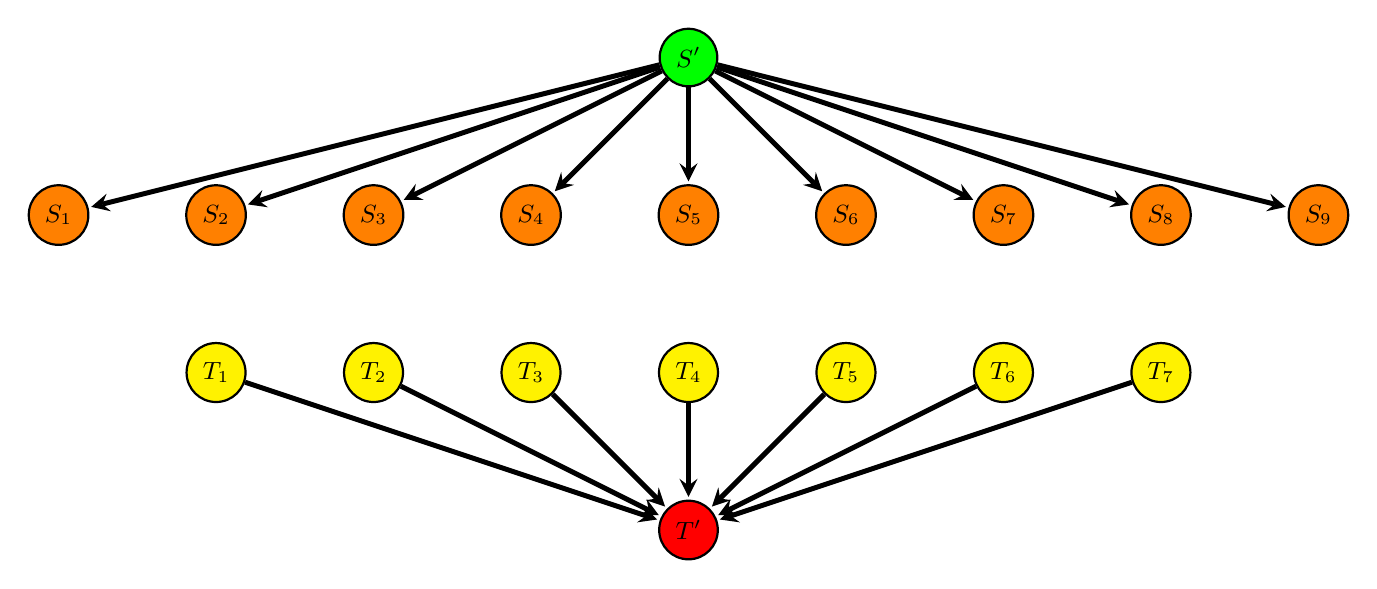
\begin{tikzpicture}[
            > = stealth, % arrow head style
            shorten > = 1pt, % don't touch arrow head to node
            auto,
            node distance = 2cm, % distance between nodes
            semithick % line style
        ]

        \tikzstyle{every state}=[
            draw = black,
            thick,
            fill = white,
            minimum size = 4mm
        ]

        \node[state, fill = orange] (b1) {$S_1$};
        \node[state, fill = orange] [right of=b1] (b2) {$S_2$};
        \node[state, fill = orange] [right of=b2](b3) {$S_3$};
        \node[state, fill = orange] [right of=b3](b4) {$S_4$};
        \node[state, fill = orange] [right of=b4](b5) {$S_5$};
        \node[state, fill = orange]  [right of=b5] (b6) {$S_6$};
        \node[state, fill = orange] [right of=b6] (b7) {$S_7$};
        \node[state, fill = orange]  [right of=b7] (b8) {$S_8$};
        \node[state, fill = orange] [right of=b8] (b9) {$S_9$};
        
        \node[state, fill = green] [above of=b5] (S) {$S'$};
        
        \node[state, fill = yellow] [below of=b2] (w1) {$T_1$};
        \node[state, fill = yellow] [right of=w1] (w2) {$T_2$};
        \node[state, fill = yellow] [right of=w2](w3) {$T_3$};
        \node[state, fill = yellow] [right of=w3](w4) {$T_4$};
        \node[state, fill = yellow] [right of=w4](w5) {$T_5$};
        \node[state, fill = yellow]  [right of=w5] (w6) {$T_6$};
        \node[state, fill = yellow] [right of=w6] (w7) {$T_7$};

        
        \node[state, fill = red] [below of=w4] (T) {$T'$};

        \path[->,line width=1.8pt] (S) edge node {} (b1);
        \path[->,line width=1.8pt] (S) edge node {} (b2);
        \path[->,line width=1.8pt] (S) edge node {} (b3);
        \path[->,line width=1.8pt] (S) edge node {} (b4);
        \path[->,line width=1.8pt] (S) edge node {} (b5);
        \path[->,line width=1.8pt] (S) edge node {} (b6);
        \path[->,line width=1.8pt] (S) edge node {} (b7);
        \path[->,line width=1.8pt] (S) edge node {} (b8);
        \path[->,line width=1.8pt] (S) edge node {} (b9);
        
        \path[->,line width=1.8pt] (w1) edge node {} (T);
        \path[->,line width=1.8pt] (w2) edge node {} (T);
        \path[->,line width=1.8pt] (w3) edge node {} (T);
        \path[->,line width=1.8pt] (w4) edge node {} (T);
        \path[->,line width=1.8pt] (w5) edge node {} (T);
        \path[->,line width=1.8pt] (w6) edge node {} (T);
        \path[->,line width=1.8pt] (w7) edge node {} (T);


  \end{tikzpicture}
\end{center}

\part Consider an example of an unweighted directed graph shown below. We need to find the maximum number of paths possible from $u$ to $v$ that do not share any {\em vertices}. 

\begin{center}
  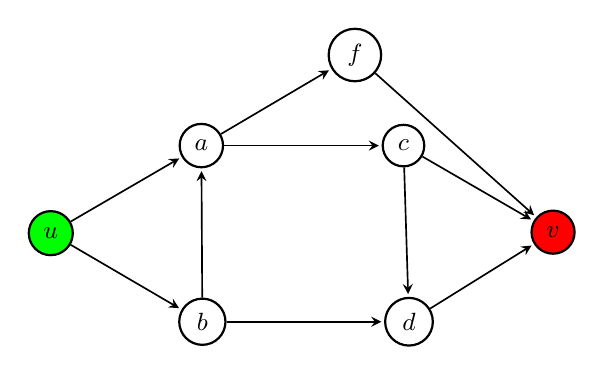
\begin{tikzpicture}[
            > = stealth, % arrow head style
            shorten > = 1pt, % don't touch arrow head to node
            auto,
            node distance = 2cm, % distance between nodes
            semithick % line style
        ]

        \tikzstyle{every state}=[
            draw = black,
            thick,
            fill = white,
            minimum size = 4mm
        ]

        \node[state, fill = green] (u) {$u$};
        \node[state] [above right=0.7cm and 1.5cm of u] (a) {$a$};
        \node[state] [right=0.7cm and 2cm of a] (c) {$c$};
        \node[state] [below right=0.7cm and 1.5cm of u] (b) {$b$};
        \node[state] [right=0.7cm and 2cm of b] (d) {$d$};
        \node[state, fill = red] [below right=0.7cm and 1.5cm of c] (v) {$v$};
        \node[state] [above right=0.7cm and 1.5cm of a] (f) {$f$};
        
        \path[->] (u) edge node {} (a);
        \path[->] (u) edge node {} (b);
        \path[->] (b) edge node {} (a);
        \path[->] (a) edge node {} (c);
        \path[->] (c) edge node {} (d);
        \path[->] (b) edge node {} (d);
        \path[->] (c) edge node {} (v);
        \path[->] (d) edge node {} (v);
        \path[->] (a) edge node {} (f);
        \path[->] (f) edge node {} (v);

  \end{tikzpicture}
\end{center}

This can be solved for the graph shown above and any unweighted directed graph by replacing every vertex other than $u$ and $v$ by a pair of vertices connected by a directed edge in a modified graph. Every edge leading into a node in the original graph, will be replaced by the same edge leading into the first node in the new node pair with the directed edge leaving the new node. Every edge leaving a node in the original graph, will be replaced by the same edge leaving the second node in the new node pair with the directed edge entering the new node. All edge weights or capacity between the new nodes will be made $1$ and the capacity between the other nodes will be made infinite. This construction is shown below: 

\begin{center}
  \begin{tikzpicture}[
            > = stealth, % arrow head style
            shorten > = 1pt, % don't touch arrow head to node
            auto,
            node distance = 2cm, % distance between nodes
            semithick % line style
        ]

        \tikzstyle{every state}=[
            draw = black,
            thick,
            fill = white,
            minimum size = 4mm
        ]

        \node[state, fill = green] (u) {$u$};
        \node[state] [above right=0.7cm and 2.75cm of u] (a1) {$a_1$};
        \node[state] [right=0.7cm and 0.5cm of a1] (a2) {$a_2$};
        \node[state] [right=0.7cm and 2cm of a2] (c1) {$c1$};
        \node[state] [right=0.7cm and 0.5cm of c1] (c2) {$c_2$};
        \node[state] [below right=0.7cm and 1.5cm of u] (b1) {$b1$};
        \node[state] [right=0.7cm and 0.5cm of b1] (b2) {$b_2$};
        \node[state] [right=0.7cm and 4.5cm of b2] (d1) {$d1$};
        \node[state] [right=0.7cm and 0.5cm of d1] (d2) {$d_2$};
        \node[state, fill = red] [below right=0.7cm and 1.5cm of c2] (v) {$v$};
        \node[state] [above right=1cm and 4.5cm of a] (f1) {$f_1$};
        \node[state] [right=0.7cm and 0.5cm of f1] (f2) {$f_2$};
        
        \path[->] (u) edge node {$\infty$} (a1);
        \path[->] (a1) edge node {1} (a2);
        \path[->] (u) edge node {$\infty$} (b1);
        \path[->] (b1) edge node {1} (b2);
        \path[->] (b2) edge node {$\infty$} (a1);
        \path[->] (a2) edge node {$\infty$} (c1);
        \path[->] (c1) edge node {1} (c2);
        \path[->] (c2) edge node {$\infty$} (d1);
        \path[->] (d1) edge node {1} (d2);
        \path[->] (b2) edge node {$\infty$} (d1);
        \path[->] (c2) edge node {$\infty$} (v);
        \path[->] (d2) edge node {$\infty$} (v);
        \path[->] (a2) edge node {$\infty$} (f1);
        \path[->] (f1) edge node {1} (f2);
        \path[->] (f2) edge node {$\infty$} (v);

  \end{tikzpicture}
\end{center}

Now if we find the max flow between $u$ and $v$, the flow through the original nodes, which have now been split into two nodes, will be restricted to one path due to the edge capacity of $1$. The max flow will end up finding the maximum number of paths possible from $u$ to $v$ that do not share any vertices. The maximum number of paths will be the result of the infinite capacity of the edges corresponding to the ones in the original graph, and since each vertex of the original graph will only be used once for a single path, the paths will not share any vertices.

\end{parts}

\titledquestion{Matchings}
Consider the matching problem that we have encountered before, but with {\em binary} weights. i.e., suppose we have $n$ children and $n$ gifts, and every child has a $0/1$ happiness value associated with each gift. The goal is to assign the gifts to the children, so as to maximize the total happiness. The question we wish to understand is: is there an assignment in which the total happiness is $n$? (I.e., can every child be assigned a gift to which he/she has a happiness value of $1$?)

\begin{parts}
\part[2] Let $\Gamma(i)$ denote the set of gifts for which child $i$ has a happiness value equal to $1$. One trivial case in which the total happiness cannot be made $n$ is if there is a set $R$ of children such that $\cup_{r \in R} \Gamma(r)$ has size $< |R|$. Give a short reason why this is so.

\part[5] Let us call a set $R$ as above a {\em trivial obstruction} (to the presence of an assignment of total happiness $n$). Prove that whenever the optimum total happiness is $<n$, such a trivial obstruction must exist. [{\em Hint:} use the max-flow min-cut theorem!] 
\end{parts}

\begin{parts}

\part Since $|\cup_{r \in R} \Gamma(r)| < |R|$, whatever kind of matching is done for the children in set $R$ there will always be some child who will not get a gift. The reason is that the size of the set of the union of gifts that each child in set $R$ likes is less than the number of children in the set $R$.

\part The matching of gifts to children can be solved by constructing a bipartite graph with nodes representing children on one side and nodes representing gifts on the other. For every gift that a child likes, construct a directed edge of capacity $1$ from the child to the gift. Put a node representing the source node on the side of the bipartite graph with the nodes representing the children. Connect the source node using directed edges of capacity $1$ to each child with the edge pointing away from the source. Construct a sink node on the other side of the graph. Connect each gift node to the sink node using directed edges of weight $1$ going into the sink. This construction is shown below:

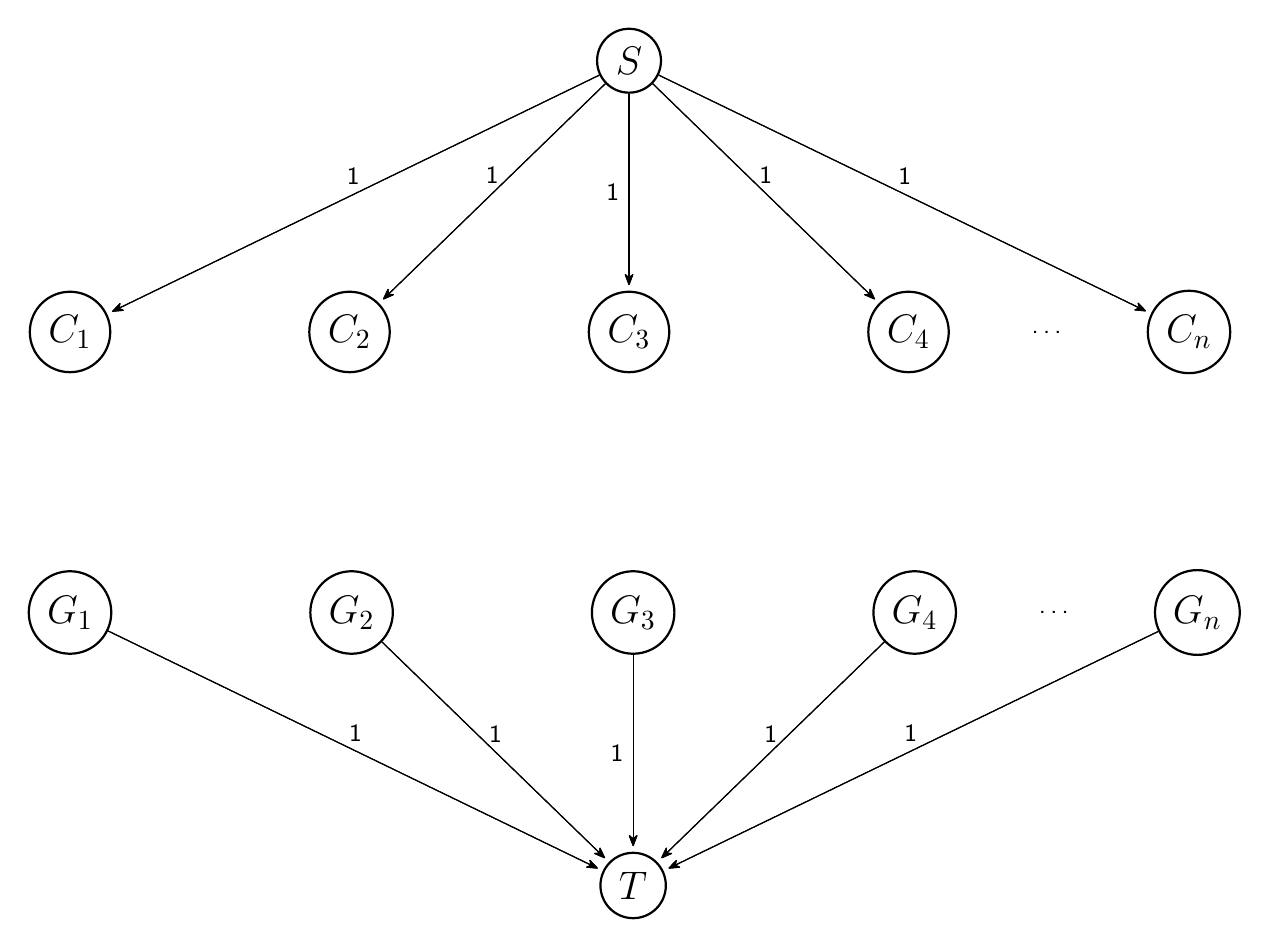
\begin{tikzpicture}[->,>={Stealth[round,sep]},shorten >=1pt,auto,node distance=2.5cm]

    \node[main node] (1) {$C_1$};
    \node[main node] (2) [right =of 1]{$C_2$};
    \node[main node] (3) [right =of 2]{$C_3$};
    \node[main node] (4) [right =of 3]{$C_4$};
    \node[main node] (5) [right =of 4]{$C_n$};
    
    \node[main node] (6) [below =of 1]{$G_1$};
    \node[main node] (7) [right =of 6]{$G_2$};
    \node[main node] (8) [right =of 7]{$G_3$};
    \node[main node] (9) [right =of 8]{$G_4$};
    \node[main node] (10) [right =of 9]{$G_n$};

    \node[main node] (11) [above =of 3]{$S$};


    \node at ($(4)!.5!(5)$) {\ldots};
    \node at ($(9)!.5!(10)$) {\ldots};

    \draw (11) -- (1);
    \draw (11) -- (1) node [midway, above] (TextNode) {1};
     \draw (11) -- (2);
    \draw (11) -- (2) node [midway, above] (TextNode) {1};
    \draw (11) -- (3);
    \draw (11) -- (3) node [midway, left] (TextNode) {1};
    \draw (11) -- (4);
    \draw (11) -- (4) node [midway, above] (TextNode) {1};
    \draw (11) -- (5);
    \draw (11) -- (5) node [midway, above] (TextNode) {1};

    \node[main node] (12) [below =of 8]{$T$};

    \draw (6) -- (12);
    \draw (6) -- (12) node [midway, above] (TextNode) {1};
    \draw (7) -- (12);
    \draw (7) -- (12) node [midway, above] (TextNode) {1};
    \draw (8) -- (12);
    \draw (8) -- (12) node [midway, left] (TextNode) {1};
    \draw (9) -- (12);
    \draw (9) -- (12) node [midway, above] (TextNode) {1};
    \draw (10) -- (12);
    \draw (10) -- (12) node [midway, above] (TextNode) {1};
   
\end{tikzpicture}
\end{parts}

The source node is represented by $S$, the child nodes are represented by $\{C_1,\ldots,C_n\}$ and the gift nodes by $\{G_1,\ldots,G_n\}$ and the sink node by $T$. The capacities of the edges going from the source node and into the sink node is shown by the number $1$ next to the directed edges. The edges between the child and gift nodes have not been shown.

We can now find the max flow from the source $S$ to the sink $T$. Since the edge capacities into the child nodes and out of the gift nodes are each $1$, the maximum flow possible will be $n$. The flow from the child to the gift nodes will correspond to one of the optimum matchings of children to gifts for maximum happiness. In case the maximum happiness found through maximum flow is less than $n$, it means that at least one child node and at least one gift node do not have any flow through them. Now consider the case when $R=\{C_1,\ldots,C_n\}$. In this case $|\cup_{r \in R} \Gamma(r)| < |R|$. If this were not the case there would have been perfect matching and maximum happiness would have been $n$. If $|\cup_{r \in R} \Gamma(r)|$ had been equal to $|R|$ ($=n$ in this case), the maximum happiness would have been $n$ since it would have been possible to find a gift for each child through max flow. So the trivial obstruction was found for the case when $R=\{C_1,\ldots,C_n\}$.

\titledquestion{Matching games}
Alice and Bob play the following game: Alice starts by naming an actress A1. Bob must then name an actor B1 who has appeared in a movie with A1. Then Alice must name an actress A2 who appeared with B1, and so on. (Alice must always pick from the set of actresses, and Bob must pick from the set of actors.) The catch is that the players are not allowed to name anyone they have named already. The game ends and a player loses if he/she cannot name an actor/actress who hasn't been named already.

Suppose we are given as input a set of all ``allowed'' movies and their casts, and suppose that the total number of actresses is equal to the total number of actors. We can construct a bipartite graph between actresses and actors, in which there is an edge iff the two have appeared together in a movie. Let us call this graph $G$.  

\begin{parts}
\part[4] Prove that if $G$ has a perfect matching, then there is a winning strategy for Bob. (I.e., no matter how Alice plays, Bob can win.)
\part[7] If $G$ does {\em not} have a perfect matching, prove that Alice has a winning strategy.  [{\em Hint:} consider small examples; start with a maximum matching, and think of how Alice might want to start the play.]
\end{parts}

\begin{parts}

\part Consider the case when there is only $1$ actor and $1$ actress. Since there is perfect matching, after Alice selects the $1$ available actress, Bob can choose the actor paired with that actress in the perfect matching. Alice will not have any more actresses to choose and thus Bob will win. This is the inductive base case. Assume that when there are $n$ pairs of actresses and actors, Bob wins. In the case when there are $n+1$ pairs, Alice has the option of choosing the actress who has appeared with the actor that Bob last chose, if there is one available. Since there is perfect matching, when Alice chooses that actress, Bob is assured that there will be an actor who has appeared with the actress last chosen by Alice. Since there are no more actresses to choose from, as all of the $n+1$ pairs have been used up, Bob will win. On the other hand, if Alice does not have an actress who has appeared with the actor that Bob last chose, Bob wins. 

Based on the above inductive proof, we can say that Bob always wins and his strategy will be to try an choose an actor such that Alice does not have an actress to choose. If that does not work, Bob will always win when they run out of actors and actresses to choose from.

\part

\end{parts}

\end{questions}

\begin{thebibliography}{9}

\bibitem{CLRS} \enquote{24. Single-Source Shortest Paths.} \textit{Introduction to Algorithms}, by Thomas H. Cormen et al., MIT Press, 2009, pp. 648-662.

\end{thebibliography}

\end{document}
